% Phys 39 Module 6 -- A3: Feedback Data and Lumped-Model Memo
% Build:  cd docs/assessments/a3 && latexmk -pdf A3.tex   (needs REVTeX 4.2; Overleaf has it)
% Figures: python docs/assessments/a3/make_figures.py   (from the repository root)
% Rename the PDF to A3_Yin.pdf before uploading to Moodle.
\documentclass[reprint, amsmath, amssymb, aps, floatfix]{revtex4-2}

\usepackage{graphicx} % Include figure files
\usepackage{dcolumn}  % Align table columns on decimal point
\usepackage{bm}       % bold math
\usepackage{url}

\newcommand{\Qdot}{\dot Q}
\newcommand{\degC}{\,^\circ\mathrm{C}}
\newcommand{\Tset}{T_{\mathrm{set}}}
\newcommand{\Tamb}{T_{\mathrm{amb}}}
\newcommand{\Tss}{T_{\mathrm{ss}}}
\newcommand{\zP}{\zeta_{\mathrm{2L,P}}}
\newcommand{\Kpc}{K_{p,\mathrm{crit}}}
\newcommand{\Kic}{K_{i,\mathrm{crit}}}

\begin{document}

\preprint{Phys 39 Module 6 -- A3}

\title{Feedback Data and Lumped Models:\\ P and PI Control of a TEC-Heated Block}

\author{Tianren Yin}
\affiliation{Physics Department, Brandeis University}

\date{\today}

\begin{abstract}
We controlled the temperature of a block heated and cooled by a thermoelectric cooler (TEC)
with P and PI feedback and compared six matched experimental runs with lumped models. A
one-lump model with the measured susceptibilities $\chi_h = 0.485$ and
$\chi_c = 0.172\degC$/PWM and time constant $\tau = 70 \pm 3$\,s predicts the P droop within
$0.13\degC$ in all six P steps, and PI control removes it. The high-gain P run overshoots
by 21\,\%, which a one-lump P model cannot do. A two-lump model with one shared parameter set
($G = 2$\,W/K, $C_T/C = 0.25$) reproduces that overshoot and orders all six responses by
$\zP$ and $\rho_I$, but it peaks 7\,s late, rings at half the measured frequency, and
over-predicts the PI overshoot by a factor of 1.5--1.7. A pure loop delay of about 3\,s
accounts for the timing. The best gains tested are $K_p = 6$\,PWM/$^\circ$C and
$K_i = 0.08$\,PWM/($^\circ$C\,s).
\end{abstract}

\maketitle

%-----------------------------------------------------------------------
\section*{1. One-lump model and P-control predictions}

\textbf{Model.} Treat the TEC, block, and thermistor as one lump at temperature $T$ with
heat capacity $C$ (J/K), coupled to the room by a conductance $H$ (W/K). The TEC supplies
$P_u$ watts per count of the signed PWM command $u$ ($u > 0$ heats, $u < 0$ cools):
\begin{equation}
C\frac{dT}{dt} = P_u u - H(T - \Tamb).
\label{eq:balance}
\end{equation}
For a constant open-loop $u$, setting $dT/dt = 0$ gives
$T_{\mathrm{ss}} - \Tamb = (P_u/H)\,u \equiv \chi u$, so $\chi = P_u/H$, with units
(W/PWM)/(W/K) $=$ K/PWM $= {}^\circ$C/PWM. Dividing Eq.~(\ref{eq:balance}) by $H$,
\begin{equation}
\tau\frac{dT}{dt} = \chi u - (T - \Tamb), \qquad \tau = \frac{C}{H}.
\label{eq:onelump}
\end{equation}
$\chi$ compares the TEC power per count with the passive conductance; it is not a ratio of
the actual heat flows, which balance at steady state. Doubling $P_u$ doubles $\chi$;
doubling $H$ halves both $\chi$ and $\tau$; doubling $C$ alone leaves $\chi$ unchanged and
doubles $\tau$. $C$ drops out of the steady state because it multiplies $dT/dt = 0$; it only
sets how fast the stored heat changes.

\textbf{Measured parameters.} The Module 4 steady-state fits give
$\chi_h = 0.485 \pm 0.007\degC$/PWM (heating) and $\chi_c = 0.172 \pm 0.002\degC$/PWM
(cooling). Four open-loop steps ($0 \to +25 \to 0 \to -25 \to 0$ PWM, 17 Oct) give 63\,\%
times of 65.6--72.7\,s, so $\tau = 70 \pm 3$\,s, the same for heating and cooling as
$\tau = C/H$ requires. The model is therefore
\begin{equation}
(70\,\mathrm{s})\,\frac{dT}{dt} = \chi u - (T - \Tamb),
\end{equation}
with $\chi = \chi_h = 0.485\degC$/PWM for $u \ge 0$ and $\chi = \chi_c = 0.172\degC$/PWM for
$u < 0$.

\textbf{P control.} With $u = K_p(\Tset - T)$, Eq.~(\ref{eq:onelump}) becomes
$\tau\,dT/dt = \chi K_p(\Tset - T) - (T - \Tamb)$. If the block were held at $\Tset$, the
command would be zero while $H(\Tset - \Tamb)$ still leaked to the room, so $T$ falls back
until the TEC heat $P_uK_p(\Tset - T)$ balances the leak $H(T - \Tamb)$. Setting
$dT/dt = 0$ and writing $\Tss - \Tamb = (\Tset - \Tamb) - (\Tset - \Tss)$,
\begin{equation}
\Tset - \Tss = \frac{\Tset - \Tamb}{1 + \chi K_p}.
\label{eq:droop}
\end{equation}
Subtracting the steady state, $\theta = T - \Tss$ obeys
$\tau\,d\theta/dt = -(1 + \chi K_p)\,\theta$, so
\begin{equation}
\tau_{\mathrm{cl}} = \frac{\tau}{1 + \chi K_p}.
\label{eq:taucl}
\end{equation}
The dimensionless loop gain is $L = \chi K_p$ [($^\circ$C/PWM)(PWM/$^\circ$C) $= 1$].
A larger $K_p$ commands more TEC power per degree of error. At steady state a smaller error
then supplies the power the room removes, so the droop is the fraction $1/(1+L)$ of the
initial error; away from steady state the same extra power per degree restores the
temperature at the faster rate $(1+L)/\tau$. Agreement requires a constant $\chi$ for the
sign of the actual command, a constant $\Tamb$, no saturation, and a settled final state.

\textbf{Comparison with measurement.} Table~\ref{tab:p} compares Eqs.~(\ref{eq:droop}) and
(\ref{eq:taucl}) with the three P runs of Sec.~2, using each run's baseline $\Tamb$ and
$\chi_h$ (every step ends with a heating command). \emph{Representative case}: in the
Run~2 upward step ($K_p = 8$, $L = 3.88$) the model predicts a droop of $2.82\degC$ and
$\tau_{\mathrm{cl}} = 14.3$\,s; we measured $2.89\degC$ and a 63\,\% time of 13.9\,s.

\begin{table}[h]
\caption{One-lump P predictions vs measurement. $t_{63}$: time after the setpoint switch
to reach 63\,\% of the step.}
\label{tab:p}
\begin{ruledtabular}
\begin{tabular}{lcccc}
Run, step & $L$ & droop pred./meas. ($^\circ$C) & $\tau_{\mathrm{cl}}$ (s) & $t_{63}$ (s) \\
\hline
1 ($K_p = 2$), up & 0.97 & 7.12 / 7.24 & 35.5 & 35.2 \\
1, down &  & 4.58 / 4.71 &  & 39.9 \\
2 ($K_p = 8$), up & 3.88 & 2.82 / 2.89 & 14.3 & 13.9 \\
2, down &  & 1.80 / 1.84 &  & 17.5 \\
3 ($K_p = 32$), up & 15.5 & 0.84 / 0.85 & 4.2 & 5.5 \\
3, down &  & 0.54 / 0.54 &  & 8.5 \\
\end{tabular}
\end{ruledtabular}
\end{table}

\emph{What agrees.} The droop follows Eq.~(\ref{eq:droop}) within $0.13\degC$ (3\,\%) in
all six steps over a 16-fold range of $K_p$, and $\tau_{\mathrm{cl}}$ agrees within 3\,\%
on the upward steps at $K_p = 2$ and 8. Only $K_p = 2$ is a genuinely small gain ($L \approx
1$ removes only half of the error). Gains must be judged in the direction of the command:
the same $K_p = 8$ gives $L = 1.38$ while cooling. The downward steps are 12--22\,\% slower: at $K_p = 8$ the
command briefly reverses (cooling, $\chi_c$), and at $K_p = 2$ it falls to 4 PWM, where the
Module 4 slope is smaller. At $K_p = 32$ the response is 1--2\,s late and
overshoots (Sec.~2), which the one-lump model cannot do (Sec.~5).

%-----------------------------------------------------------------------
\section*{2. Experimental Goldilocks plots and step-response metrics}

All six runs use the same apparatus and protocol: control starts from room temperature
($\Tamb = 20.98$--$22.02\degC$) with $\Tset = 30\degC$, then the setpoint is switched to
$35\degC$ and back to $30\degC$ after each response has settled; $u_{\max} = 255$,
anti-windup on, the integral zeroed before each PI run, and one reading every 1.08\,s.
The P runs use $K_p = 2$, 8, 32\,PWM/$^\circ$C; the PI runs share $K_p = 6$ with
$K_i = 0.04$, 0.08, 0.5\,PWM/($^\circ$C\,s) (Fig.~\ref{fig:exp}).

\begin{figure*}
\centering
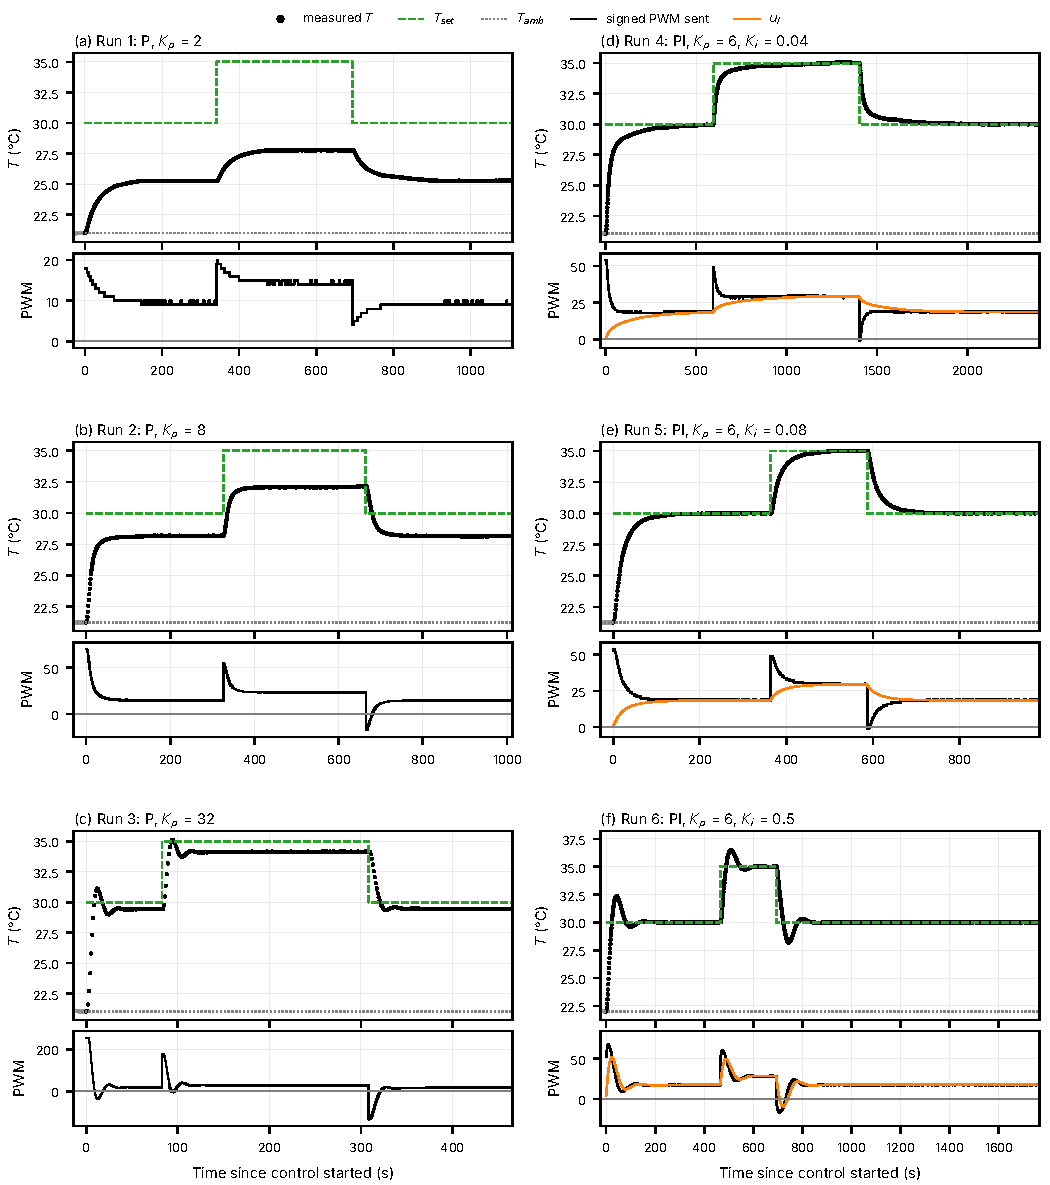
\includegraphics[width=\textwidth]{figures/exp_grid.pdf}
\caption{Six experimental Goldilocks runs. Upper panels: measured temperature (output $y$,
black; grey: baseline before control), setpoint (green dashed), and $\Tamb$ (dotted).
Lower panels: signed PWM sent (input $u$; heating positive) and, for PI, the integral
contribution $u_I = K_iq$ (orange). (a)--(c) P control: the droop falls as $1/(1+L)$ and
the response speeds up; $K_p = 32$ overshoots and rings once. (d)--(f) PI control: the droop
is removed in every run, with $u_I$ holding the steady command (18--29 PWM) at $e = 0$;
$K_i = 0.04$ creeps to the setpoint in 7--9 min, $K_i = 0.08$ settles in about 2 min without
overshoot, $K_i = 0.5$ overshoots by 1.5--1.8$\degC$ and rings.}
\label{fig:exp}
\end{figure*}

\textbf{Metrics} (Table~\ref{tab:metrics}; \path{python/module6_a3_metrics.py}). For each
step, $T_{\mathrm{start}}$ is the mean of the last 30\,s before the switch and $\Tss$ the
mean of the last 60\,s of the step. \emph{Rise time}: 10\,\% to 90\,\% of
$\Tss - T_{\mathrm{start}}$ (first crossings, interpolated). \emph{Percent overshoot}: first
extreme past $\Tss$ divided by the step. \emph{Settling time}: from the switch until $T$
stays within $\Tss \pm 0.1\degC$ (2\,\% of the $5\degC$ step; the reading noise is
0.005--0.02$\degC$ rms). \emph{Steady-state error}: $e_{ss} = \Tset - \Tss$.
\emph{Period}: time between the first two extremes on the overshoot side, or twice the time
from the first extreme to the opposite one; extremes count only if more than $0.05\degC$
past $\Tss$.

\begin{table}[h]
\caption{Step-response metrics of the largest-gain P (Run 3, $K_p = 32$) and PI (Run 6,
$K_p = 6$, $K_i = 0.5$) runs. Up: $30 \to 35\degC$; down: $35 \to 30\degC$.}
\label{tab:metrics}
\begin{ruledtabular}
\begin{tabular}{lcccccc}
 & Rise & \multicolumn{2}{c}{Overshoot} & Settling & $e_{ss}$ & Period \\
 & (s) & (\%) & ($^\circ$C at s) & (s) & ($^\circ$C) & (s) \\
\hline
P, up & 4.8 & 20.5 & 0.97 at 11.8 & 28 & $+0.85$ & 19.4 \\
P, down & 9.9 & 1.9 & 0.09 at 18.3 & 32 & $+0.54$ & 17\footnotemark[1] \\
PI, up & 15.8 & 29.7 & 1.48 at 43.0 & 122 & 0.00 & 105 \\
PI, down & 20.0 & 36.1 & 1.81 at 50.6 & 130 & 0.00 & 116 \\
\end{tabular}
\end{ruledtabular}
\footnotetext[1]{One weak rebound ($0.13\degC$); barely above the threshold.}
\end{table}

The P command peaks at $+178$ PWM (up) and $-133$ PWM (down) and the PI command never
exceeds 68 PWM, so none of these steps saturates (only the first three readings of the
Run~3 approach from room temperature are at 255). The high-gain P step is fast but keeps a
$0.5$--$0.9\degC$ droop; the high-gain PI step has no droop but overshoots more and settles
four times more slowly. Heating and cooling differ: the P downward step, whose large
command is cooling, rings less (loop gain $\chi_cK_p = 5.5$ instead of $\chi_hK_p = 15.5$),
while the PI downward step overshoots more (lower one-lump $\zeta_c$).

%-----------------------------------------------------------------------
\section*{3. Simulation Goldilocks plots and comparison}

\textbf{Shared parameters.} All six simulations use the course two-lump model
(\path{python/Lab_6_7_modeling_tec.py}) in \texttt{measured} mode with
$\chi_c = 0.172$ and $\chi_h = 0.485\degC$/PWM, $\tau = 70$\,s, $V_{\mathrm{TEC}} = 10.95$\,V,
and $R_M = 1.50\,\Omega$ (which give $C = 70.1$\,J/K, $H = 1.00$\,W/K,
$P_{u,c} = 0.172$\,W/PWM, $r = 2.82$), with $G = 2$\,W/K, $C_T/C = 0.25$, a PWM limit of 255,
anti-windup on, $\Delta t = 0.05$\,s, and each run's own baseline $\Tamb$, initial
temperature, and setpoint switch times; only the controller mode, $K_p$, and $K_i$ change.
The room differed by up to $1.0\degC$ between runs, so each simulation starts, like its
experiment, from the measured room temperature; with one common $\Tamb = 21.05\degC$ the P
droops would move by at most $0.04\degC$.
$G$ and $C_T/C$ were chosen once, from the Run~3 upward step: $G = 2$ and 3\,W/K bracket its
$0.97\degC$ overshoot (1.09 and $0.79\degC$; the field takes whole numbers), and at $G = 2$
the fraction $C_T/C = 0.25$ gives $0.98\degC$
(Fig.~\ref{fig:sim}; \path{python/module6_part2_goldilocks.py}).

\begin{figure*}
\centering
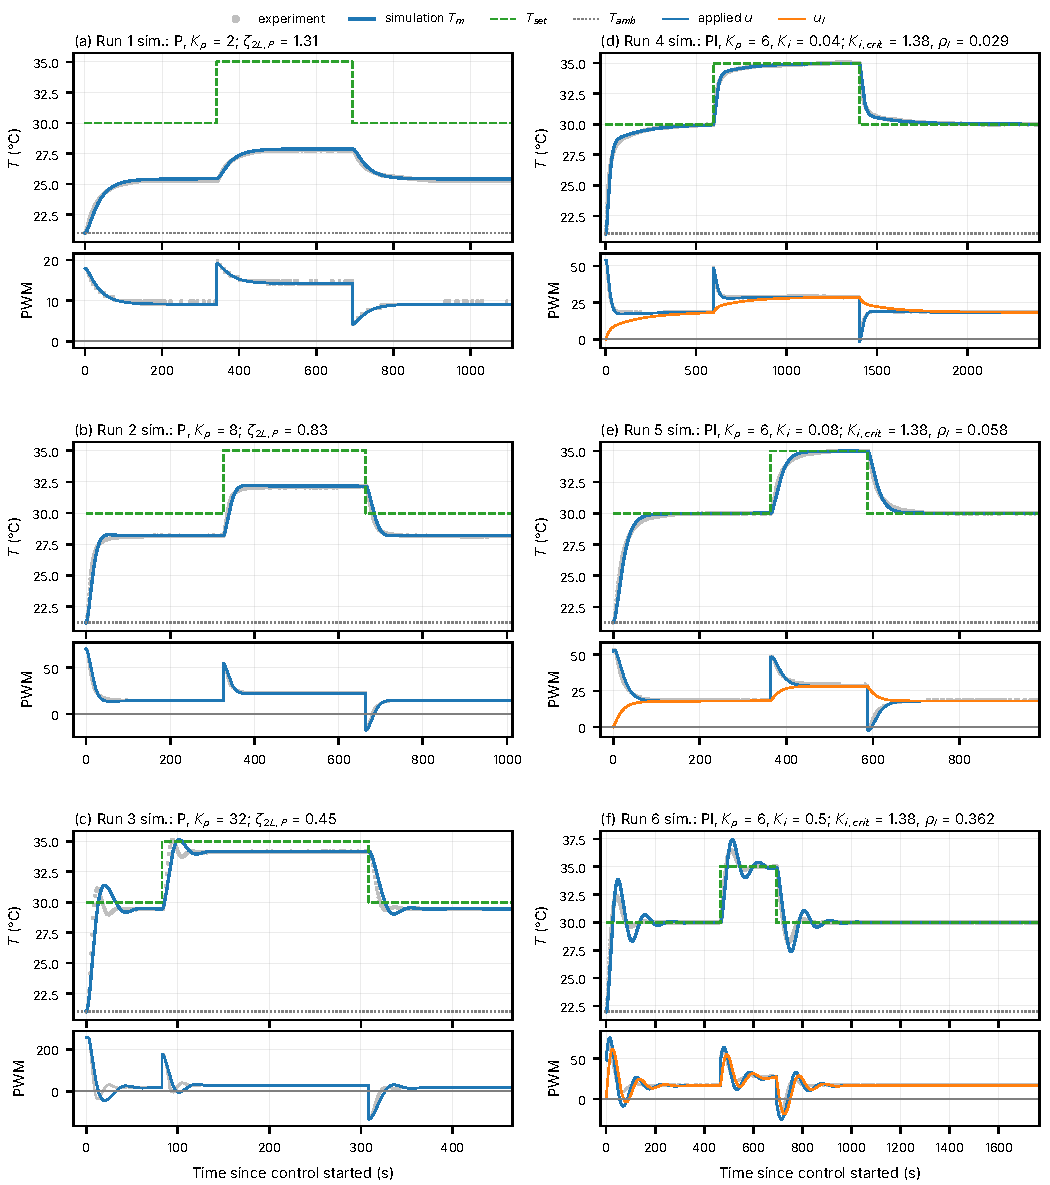
\includegraphics[width=\textwidth]{figures/sim_grid.pdf}
\caption{Six two-lump simulations with the shared parameters, on the same axes as
Fig.~\ref{fig:exp} (grey: experiment). Blue: simulated mass temperature $T_m$ and applied
signed PWM; orange: $u_I$. (a)--(c) P: displayed $\zP = 1.308$, 0.831, 0.452 for
$K_p = 2$, 8, 32; $\Kpc = 4.89$\,PWM/$^\circ$C. (d)--(f) PI with $K_p = 6$: displayed
$\Kic = 1.38$\,PWM/($^\circ$C\,s) and $\rho_I = K_i/\Kic = 0.029$, 0.058, 0.362 for
$K_i = 0.04$, 0.08, 0.5.}
\label{fig:sim}
\end{figure*}

\begin{table*}
\caption{Measured / simulated step metrics (same definitions as Table~\ref{tab:metrics}); PI runs have $K_p = 6$.}
\label{tab:simcomp}
\begin{ruledtabular}
\begin{tabular}{lllccccc}
Run & Gains & Stability & Step & Rise (s) & Overshoot ($^\circ$C) & Settling (s) & Period (s) \\
\hline
1 & P, $K_p = 2$ & $\zP = 1.31$ & up & 77 / 75 & 0.02 / 0 & 106 / 113 & -- \\
 & &  & down & 119 / 75 & 0.06 / 0 & 176 / 113 & -- \\
2 & P, $K_p = 8$ & $\zP = 0.83$ & up & 27 / 25 & 0.05 / 0.04 & 67 / 38 & -- \\
 & &  & down & 31 / 29 & 0.05 / 0.03 & 70 / 44 & -- \\
3 & P, $K_p = 32$ & $\zP = 0.45$ & up & 4.8 / 8.1 & 0.97 / 0.98 & 28 / 44 & 19 / 37 \\
 & &  & down & 9.9 / 14.2 & 0.09 / 0.43 & 32 / 37 & 17 / 37 \\
4 & PI, $K_i = 0.04$ & $\rho_I = 0.029$ & up & 131 / 111 & 0.08 / 0 & 530 / 391 & -- \\
 & &  & down & 115 / 102 & 0.02 / 0 & 418 / 392 & -- \\
5 & PI, $K_i = 0.08$ & $\rho_I = 0.058$ & up & 56 / 42 & 0.01 / 0 & 119 / 76 & -- \\
 & &  & down & 55 / 42 & 0.02 / 0 & 116 / 75 & -- \\
6 & PI, $K_i = 0.5$ & $\rho_I = 0.362$ & up & 16 / 18 & 1.48 / 2.46 & 122 / 215 & 105 / 105 \\
 & &  & down & 20 / 22 & 1.81 / 2.63 & 130 / 236 & 116 / 106 \\
\end{tabular}
\end{ruledtabular}
\end{table*}

\textbf{Stability measures and classification.} The two-lump P loop is second order with
positive coefficients, so it is stable for every $K_p$ and becomes underdamped above
$\Kpc = 4.89$\,PWM/$^\circ$C. $K_p = 2$ lies below $\Kpc$ (stable non-oscillatory),
$K_p = 8$ just above it (stable underdamped; the 0.03--0.06$\degC$ overshoot is at the noise
level in the experiment), and $K_p = 32$ far above it (stable underdamped, one overshoot and
one ring). Decreasing $\zP$ shortens the rise (75 $\to$ 25 $\to$ 8\,s simulated, 77 $\to$ 27
$\to$ 5\,s measured) and brings overshoot. The PI loop is third order and stable only for
$\rho_I < 1$; all three runs are far below 1, so the model permits no marginal or unstable
run, and none was observed. Runs~4 and 5 are stable non-oscillatory, Run~6 stable
underdamped. Increasing $\rho_I$ shortens the rise (111 $\to$ 42 $\to$ 18\,s) and turns a
creeping approach into a ringing one; settling is shortest at the middle value. At these
small $\rho_I$ the overshoot of Run~6 comes mainly from the PI zero (one-lump
$\zeta_h = 0.47$), not from the stability limit. The decay follows the same measures: the
first rebound is 0.20 of the overshoot at $\zP = 0.45$ (Run~3) and 0.39 at $\rho_I = 0.36$
(Run~6) in the simulation, but 0.43 and 0.17 in the experiment. The real high-gain P loop is
less damped than the model and the slow PI loop more, which points to a delay (Sec.~5).

\textbf{Guided comparison.} (1)~\emph{Best matches}: Run~2 among the P runs (rise within
about 2\,s, droop within $0.07\degC$, no visible overshoot), and Runs~4 and 5 among the PI runs
(the curves overlie, both without overshoot; the simulation is 10--25\,\% faster). Run~6 is
the poorest match. (2)~The P responses are ordered by $\zP$ and their position relative to
$\Kpc$, as above. (3)~The PI responses are ordered by $\rho_I$, as above.
(4)~\emph{Agreement}: the steady state, which does not depend on $G$: the P droop agrees
within $0.13\degC$, the PI error goes to zero with the same steady command (within about
1--2 PWM), and the ordering by $\zP$ and $\rho_I$ is the same in experiment and
simulation; the Run~6 period also agrees (105\,s). \emph{Disagreement}: the time scale of the
high-gain ringing. Run~3 peaks 11.8\,s after the step with a 19\,s period; the simulation
peaks at 18.7\,s with a 37\,s period, and a scan over $G = 1$--15\,W/K and
$C_T/C = 0.05$--0.95 found no pair that peaks before 13.6\,s. The model also over-predicts
the Run~3 downward undershoot (0.43 vs 0.09$\degC$) and the Run~6 overshoot by a factor of
1.5--1.7. No shared pair fits both oscillating runs: at $C_T/C = 0.25$, Run~6 needs
$G \approx 8$\,W/K, where Run~3 overshoots by only $0.05\degC$
(Fig.~\ref{fig:compare}). This falsifies the two-lump model as the complete source of the
lag (Sec.~5).

\begin{figure}[t]
\centering
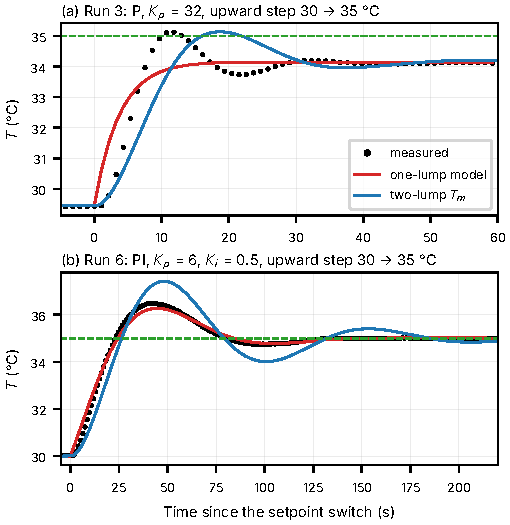
\includegraphics[width=\columnwidth]{figures/model_compare.pdf}
\caption{Upward steps of (a) Run~3 and (b) Run~6: measured, one-lump model (red; same
gains, integer PWM, one-reading command delay), and two-lump $T_m$ with the shared
parameters (blue). The one-lump model cannot overshoot in (a); the two-lump model
overshoots by the right amount but late, and too much in (b).}
\label{fig:compare}
\end{figure}

%-----------------------------------------------------------------------
\section*{4. PI steady state, assumptions, and windup}

\textbf{Ideal steady state.} The controller is
\begin{equation}
u = u_P + u_I = K_pe + K_iq, \qquad \frac{dq}{dt} = e = \Tset - T.
\end{equation}
At any steady state $dq/dt = 0$, so $e = 0$: for $\Tset = 55\degC$, $\Tss = 55\degC$
exactly, whatever $K_p$, $K_i$, $\chi$, or $\Tamb$. The command is then carried entirely by
the integral: $u_P = 0$ and $u_I = K_iq_{ss} = (\Tset - \Tamb)/\chi_h$, which is
$(55 - 21)/0.485 = 70$\,PWM from a $21\degC$ room (for $K_i = 0.08$,
$q_{ss} = 876\degC$\,s). P control needs a nonzero error to produce this command, hence the
droop of Eq.~(\ref{eq:droop}); the integral term supplies it from the stored error, so the
error can vanish. Our PI runs confirm this: $e_{ss} = 0.00$--$0.02\degC$ in all six PI steps,
with $u_I$ equal to the required 18--29 PWM.

\textbf{Conditions.} The result holds only if: (i)~the closed loop is stable, so a steady
state exists (one-lump PI is stable for all $K_i > 0$; with internal lag we need
$\rho_I < 1$); (ii)~the required command is within the PWM range \emph{and} in the available
direction ($70 < 255$, heating); (iii)~the actuator is not saturated at steady state; a
transient may saturate, but the integral must not be frozen or wound up when it ends;
(iv)~the integral keeps acting (it is not reset, and anti-windup releases it once out of
saturation); and (v)~the measured temperature is the true block temperature, because PI
drives the \emph{measured} error to zero: a thermistor offset becomes a steady error of the
block, and noise is averaged but not removed. At $55\degC$ the Arduino's $60\degC$ shutdown
also limits the transient: a linear 30\,\% overshoot (Run~6 gains) of a $34\degC$ step
from room would pass $60\degC$, so gains without overshoot (Run~5) are required.

\textbf{Windup and anti-windup.} The requested command
$u_{\mathrm{req}} = K_pe + K_iq$, with $q_{n+1} = q_n + e_n\Delta t$, is clamped to
$\pm u_{\max}$. If a large error asks for more than $u_{\max}$, the TEC cannot respond more,
but plain integration keeps adding error to $q$. That stored integral has no effect while
the command is clipped; when $T$ reaches $\Tset$, $u_P \to 0$ but $u_I$ is still large, so
the TEC keeps driving through the setpoint until error of the opposite sign unwinds $q$:
extra overshoot and slow recovery. Our rule is \emph{conditional integration}
(\path{python/module6_pi_control_gui.py}, \texttt{pi\_control}, lines 133--137): if
$K_pe + K_iq_{n+1}$ is beyond $\pm u_{\max}$ and $e$ pushes it farther, keep $q_n$;
otherwise integrate, including when $e$ brings the command back. In simulation with
$u_{\max} = 30$ (Part I, Part 6, one-lump, $K_p = 8$, $K_i = 0.36$) the overshoot was
$0.20\degC$ with anti-windup and $3.27\degC$ without, with $q$ peaking at 67 vs 343$\degC$\,s
($q_{ss} = 58\degC$\,s). In the hardware PI runs the command never exceeded 68 PWM, so the
rule never engaged. The clamp, the rule, and the Arduino shutdown have different jobs:
protect the actuator, limit the controller's memory, and protect the apparatus.

\textbf{Resetting the integral at steady state.} Setting $q = 0$ removes $u_I$; with
$e = 0$ the command drops to zero, so the block starts cooling toward $\Tamb$ at an initial
rate $(\Tset - \Tamb)/\tau$. The error grows, $u_P$ responds at once, and $q$ rebuilds until
$u_I$ again carries the whole command; the temperature dips and recovers like a
disturbance (Part I, Part 6: a $1.71\degC$ dip 37\,s after the reset at $30\degC$; the dip
scales with $\Tset - \Tamb$).

%-----------------------------------------------------------------------
\section*{5. Model limits and gain selection}

\textbf{The one-lump P model cannot overshoot.} With $\theta = T - \Tss$, P control gives
$d\theta/dt = -\theta/\tau_{\mathrm{cl}}$, so $\theta(t) = \theta(0)\,e^{-t/\tau_{\mathrm{cl}}}$.
The only eigenvalue, $-(1+L)/\tau$, is real and negative for every $K_p \ge 0$; $\theta$
never changes sign, and $dT/dt = -\theta/\tau_{\mathrm{cl}}$ cannot change sign either. $T$
approaches $\Tss$ monotonically from one side: no overshoot, ringing, or oscillation at any
gain. Run~3 (21\,\% overshoot, Fig.~\ref{fig:compare}a) therefore shows a missing state.

\textbf{Internal lag.} Split the lump into the TEC side ($C_T$, $T$) and the measured mass
($C_m$, $T_m$), joined by $G$:
\begin{align}
C_T\frac{dT}{dt} &= P_uu - G(T - T_m),\\
C_m\frac{dT_m}{dt} &= G(T - T_m) - H(T_m - \Tamb).
\end{align}
Heat enters $C_T$ first and reaches the thermistor only through $G$, so $T_m$ lags $T$.
When $T_m$ reaches the setpoint, the TEC side is still hotter and its stored heat
$C_T(T - T_m)$ keeps flowing into the mass: the overshoot (in the Run~3 simulation the TEC
side reaches $52\degC$ while $T_m$ approaches $30\degC$). With $u = K_p(\Tset - T_m)$,
eliminating $T$ gives one second-order equation,
\begin{multline}
C_TC_m\ddot T_m + [C_T(G+H) + C_mG]\dot T_m + G(H + P_uK_p)\,T_m \\
= G(P_uK_p\Tset + H\Tamb),
\end{multline}
with damping ratio
$\zP = [C_T(G+H) + C_mG]/[2\sqrt{C_TC_mG(H + P_uK_p)}]$, which falls below 1 for
$K_p > \Kpc = P_u^{-1}\{[C_T(G+H) + C_mG]^2/(4C_TC_mG) - H\}$. With PI the characteristic
equation is
$C_TC_ms^3 + [C_T(G+H) + C_mG]s^2 + G(H + P_uK_p)s + GP_uK_i = 0$; the Routh--Hurwitz
condition gives stability for
$K_i < \Kic = [C_T(G+H) + C_mG](H + P_uK_p)/(C_TC_mP_u)$. The twelve plots show what this
adds: the one-lump model reproduces the steady states and the low-gain runs, but only a
lagged state produces the Run~3 ringing, and the PI overshoot of Run~6 grows with the lag.

\textbf{Final gains.} We choose PI with $K_p = 6$\,PWM/$^\circ$C and
$K_i = 0.08$\,PWM/($^\circ$C\,s) (Run~5). $K_p = 6$ is just above $\Kpc = 4.89$
($\zP = 0.93$), so the proportional part is fast without ringing. $\rho_I = 0.058$ keeps the
loop far from the stability limit, and $K_i \approx K_p/\tau = 0.086$ places the PI zero on the
slow pole (one-lump $\zeta_h = 1.19$), so the integral removes the droop without
overshoot: $e_{ss} = 0$, settling in about 2\,min. $K_i = 0.04$ ($\rho_I = 0.029$) takes four
times longer; $K_i = 0.5$ ($\rho_I = 0.36$) rises faster but overshoots by 30--36\,\% and
settles no sooner. A larger $K_p$ would be faster, but Run~3 shows that at $6.5\Kpc$ the
real loop already overshoots by 21\,\% under P alone, and the missing delay (below) makes the
real margin smaller than the model suggests.

\textbf{What a better model needs: loop delay.} A pure delay $t_d$ in the command path
(half of each 1.08\,s sample, the command applied one reading later, and the 1--2\,s thermal
delay seen in the open-loop steps) costs phase in proportion to frequency, so it matters for
the fast Run~3 loop (period $\approx 20$\,s) much more than for the slow Run~6 loop
($\approx 110$\,s), whereas a heat store with $G = 2$\,W/K slows both alike. A one-lump model
with $t_d = 3$\,s and no second lump (\path{python/module6_a3_delay_check.py}) gives for
Run~3 an upward overshoot of $0.86\degC$ at 10.7\,s with a 17\,s period and a downward
undershoot of $0.12\degC$ (measured 0.97$\degC$ at 11.8\,s, 19\,s, 0.09$\degC$), and for Run~6
1.72 and 2.09$\degC$ (measured 1.48 and 1.81$\degC$; two-lump 2.46 and 2.63$\degC$). The delay
reproduces the timing that no $(G, C_T/C)$ pair can; a model with a delay of about 2--3\,s
and a weaker second lump is the next step.

%-----------------------------------------------------------------------
\section*{Data and code}

{\footnotesize\raggedright
Repository \url{https://github.com/tyin-source/__Lab_Module_6__}, modeling checkpoint
commit \texttt{0ebd3a5}. Runs 1--6: \path{data/module_06/} (the six files are listed in its
\path{README.md}, with the debugging runs). Controller: \path{python/module6_pi_control_gui.py} and
\path{arduino/module6_pi_control/}. Analysis (\path{python/}):
\path{module6_part7_runs.py}, \path{module6_a3_metrics.py}
(Tables~\ref{tab:p}--\ref{tab:simcomp}), \path{module6_part2_goldilocks.py},
\path{module6_a3_delay_check.py}; figures: \path{docs/assessments/a3/make_figures.py}.
Derivations, GUI explorations, and run notes: \path{docs/module_notes/module_06_pi_control.md}
(Part I) and \path{module_06_part2_two_lump.md} (Part II).

\textbf{AI use.} I made all hardware runs and GUI simulations and chose the run conditions
and gains. Claude Code (an AI coding assistant) wrote the GUI, the analysis and figure
scripts, and drafted this memo from my data and module notes; I reviewed the text and checked
the numbers against the data.
\par}

\end{document}
